
%%%%%%%%%%%%%%%%%% CONCLUSIONES %%%%%%%%%%%%%%

En el presente trabajo se logró diseñar e implementar satisfactoriamente un amplificador de audio clase~G. El trabajo consistió de varias etapas, entre ellas: diseño del amplificador por etapas (entrada, amplificación, potencia), simulación, en donde se tuvieron que modificar cuestiones del diseño para que cumplan las especificaciones correspondientes a un amplificador de audio. Una vez finalizadas las pruebas, se prosiguió por implementar el circuito diseñado usando \textit{Kicad} para diseñar el PCB, que luego fue fabricado y soldado.\\

Además, se diseño y construyó correctamente una fuente \textit{Switching}, encargada de entregar las tensiones necesarias para el funcionamiento del amplificador, de modo que sea utilizada una única fuente de laboratorio.\\


Finalmente, se destaca la eficiencia de este amplificador, como también su baja distorsión y su respuesta en frecuencia. 







\begin{figure}[H]
    \centering
    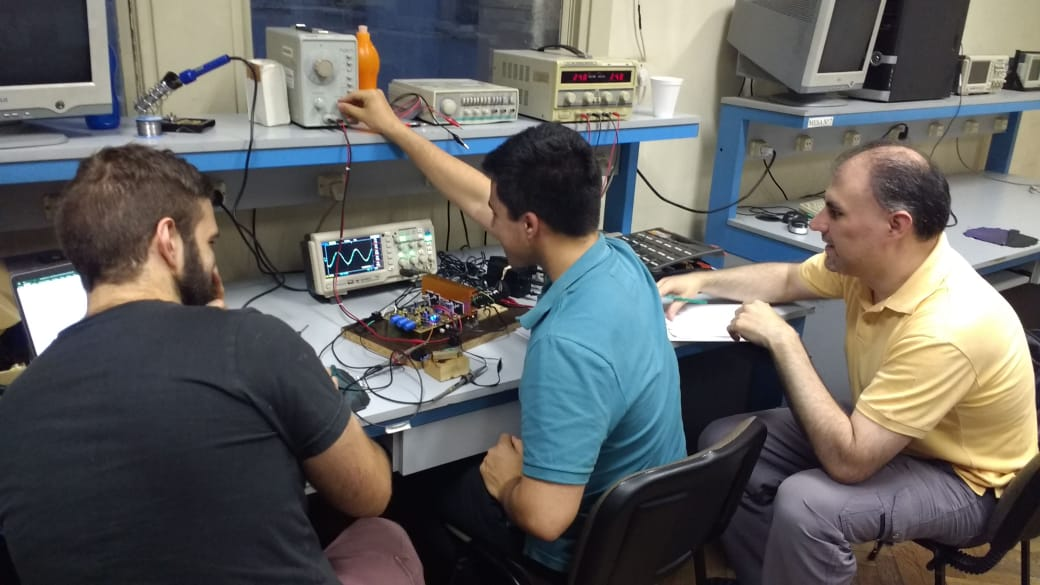
\includegraphics[scale=.4]{img/fotos/Dream_Team.jpeg}
    \caption{Último día de mediciones.}
    \label{fig:grupo_midiendo}
\end{figure}